\chapter{Desarrollo.}
\section{Instalación del servidor PowerTAC y conexión con el broker Sample}

Como parte de la actividad de estudio de la plataforma PowerTAC, fue necesario familiarizarse con el servidor, aprender su configuración básica, y la configuración necesaria para conectarse a uno o varios brokers para hacer que compitan, a su vez, familiarizarse con el ambiente de desarrollo de un broker y su configuración para conectarse a un servidor. A continuación se muestra un resumen de la investigación que se hizo sobre la plataforma.
%no se si sea necesario
\subsection{Power TAC}

Power TAC es una competencia anual que se ha realizado desde 2012, donde se simulan futuros mercados minoristas liberados de energía eléctrica, en la que los competidores son entidades de negocios o ``Brokers'' (En la simulación son agentes Inteligentes) minoristas que compran y venden energía tanto en los mercados al por mayor como al por menor.

Los brokers ofrecen servicios de energía a los clientes a través de contratos tarifarios, y luego deben servir a esos clientes negociando esa energía en el mercado al por mayor. En la competencia los brokers son desafiados a maximizar sus ganancias comprando y vendiendo energía en los mercados mayorista y minorista, sujetos a costos fijos y restricciones, el ganador de un juego o simulación individual es el broker con el saldo bancario más alto al final de la simulación \cite{WKetterJCollinsyMdWeerdtThe2017PowerTAC}.

El mercado minorista está integrado por consumidores y productores pequeños, tales como hogares, pequeñas y medianas empresas, propietarios de vehículos eléctricos, etc. es un mercado de tarifas, en el que los clientes pueden elegir entre ofertas de contratos tarifarios de los brokers competidores, comprando pequeñas cantidades de energía (pequeñas en contraste con el mercado al por mayor).

En el mercado al por mayor los brokers interactúan entre si directamente así como con grandes compañías productoras y otros participantes del mercado al por mayor vendiendo y comprando grandes cantidades de energía, la cual usan para venderla en el mercado al por menor. Los clientes son modelos de usuarios domésticos, empresariales e institucionales de energía eléctrica, así como productores de energía que poseen paneles solares o turbinas eólicas.

\subsection{Servidor}

Debido a que se trata de un proyecto de Maven, lo primero que se hizo fue instalarlo, para esto se descargó de su página oficial el paquete de instalación en un archivo zip: \textsf{http://maven.apache.org/download.cgi}
Para instalarlo, basta con descomprimirlo en la carpeta deseada, en este caso el directorio de instalación elegido fue:\\ \texttt{/usr/local/apache-maven-3.3.9}, 
para usarlo en la terminal, fue necesario agregar la carpeta de instalación: \texttt{/usr/local/apache-maven-3.3.9/bin} 
a la variable de entorno path del sistema.

Para esto se agregó la dirección de la carpeta de instalación a los archivos:\\
\texttt{/etc/environment y /etc/profile}, para resultados inmediatos se usó el comando:\\
\texttt{export PATH=\$PATH:/usr/local/apache-maven-3.3.9/bin}\\

Una vez instalado el software Maven, el siguiente paso fue descargar el archivo zip del proyecto de este enlace:\\ \textsf{https://github.com/powertac/server-distribution/releases/tag/v1.3.2}\\
Al terminar la descarga se descomprimió el archivo zip en la carpeta de trabajo\\
\texttt{/home/Documentos/power tac/} \\
Para ejecutar el servidor nos movemos al directorio raíz del proyecto y escribimos el comando correspondiente al modo que queremos ejecutar, el simulador dispone de tres modos: el modo bootstrap, el modo simulación y el modo web.

\begin{enumerate}
	\item \textbf{Bootstrap:} Es necesario correr este modo previamente a la simulación, en este modo se genera un archivo de datos bootstrap, el cual sirve como datos preliminares para ejecutar el modo simulación, este archivo contiene información del clima, información del mercado de tarifas entre otras cosas.

	\item \textbf{Simulación:} Inicia la simulación de entorno donde varios brokers se conectan al servidor y compiten entre sí.
	\item \textbf{Web: } Despliega un servidor web por el cual se puede arrancar cualquiera de los dos modos del servidor anteriores usando una interfaz gráfica amigable, además en el modo simulación dispone de una herramienta de visualización.
\end{enumerate}

Para correr el simulador en modo bootstrap se usó el siguiente comando:\\
\texttt{mvn -Pcli -Dexec.args=``--boot bootstrap-data ''}\\
Donde \texttt{bootstrap-data} es el nombre que se le pondrá al archive generado.
Para correr el servidor en modo simulación se usó el siguiente comando:\\
\texttt{mvn -Pcli -Dexec.args=``--sim --boot-data bootstrap-data ''}

Una vez más \texttt{bootstrap-data} es el nombre del archivo generado por el modo bootstrap. Hay más parámetros para correr el servidor y estos se toman por default del archivo server.properties el cual contiene la configuración por defecto, algunos de estos parámetros de configuración aparecen en la tabla que aparece en la figura \ref{tab:parametros}.

Por último el comando para desplegar el servidor web es el siguiente:
\texttt{mvn -P web}

Al entrar en la interfaz web del servidor podemos ver que nos muestra un formulario para iniciar cualquiera de los modos anteriores (bootstrap o simulación), este formulario se muestra en la figura \ref{fig:interfazFormularioWeb}.

Para correr el modo simulación desde la interfaz web se pusieron los parámetros de la \ref{tab:parametros}.

\begin{table}[!h]
	\begin{center}
		\begin{tabular}{|p{2.5cm}|p{7cm}|p{4cm}|}\hline
			\textbf{Parámetro} & \textbf{Descripción} & \textbf{Valor} \\ \hline
				Input Bootstrap data:  &El nombre del archivo xml generado en el modo bootstrap. & \texttt{bootstrap-data} \\ \hline
				JMS URL: & La url del JMS del broker, este es el valor default. & \texttt{tcp://localhost:61616} \\\hline
				Brokers  & El nombre de usuario del o los brokers que el servidor esperara a que se conecten. & \texttt{Sample}
			\\ \hline
		\end{tabular}			
	\end{center}
	\caption{ Parámetros del servidor.}
	\label{tab:parametros}
\end{table}

%imagen 

\begin{figure}[!h]
	\centering
	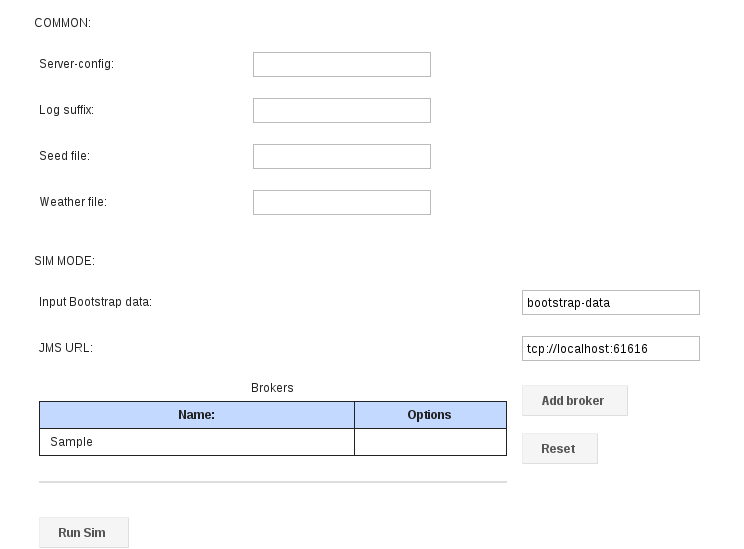
\includegraphics[width=13cm]{img/interfazFormularioWeb.png}
	\caption{Interfaz web del servidor powerTAC}
	\label{fig:interfazFormularioWeb}
\end{figure}

Los otros parámetros (Server-config, Log suffix, Seed file, Weather file) se dejaron en blanco y toman valores por defecto, para propósitos de esta prueba no son necesarios.

Una vez listos los parámetros se inició la sesión dando click en el boton Run Sim, justo abajo del formulario de los parámetros, esto inicia el simulador pero no empieza la simulación %(muestra el mensaje “simulation started”) 
(muestra el mensaje ``simulation started'') 
es decir, no inicio el juego, ya que el servidor quedo en espera del broker Sample.

\subsection{Broker}
Debido a que el broker es en lo que se trabajará agregando funcionalidades, se decidió usar un IDE para tener un buen ambiente de desarrollo, y no solo manejarlo desde la consola como se hizo con el servidor. El IDE elegido para esta prueba fue NetBeans.
Para descargar el broker de ejemplo se usó la herramienta integrada en NetBeans para descargar directamente del repositorio GitHub usando este enlace: \textsf{https://github.com/powertac/sample-broker}\\
En la figura \ref{fig:asistenteNetbeansClonar} se muestra la ventana del asistente de NetBeans para clonar repositorios desde un servidor git.

\begin{figure}[h]
	\centering
	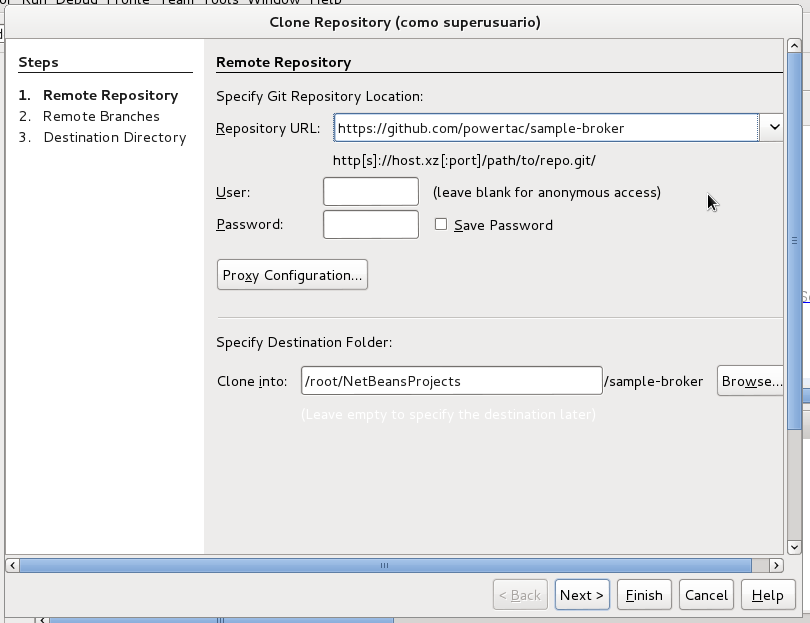
\includegraphics[width=13cm]{img/asistenteNetbeansClonar.png}
	\caption{Asistente de NetBeans para clonar proyectos desde un servidor git.}
	\label{fig:asistenteNetbeansClonar}
\end{figure}

Los parámetros de configuración del broker pueden ponerse en los argumentos a la hora de ejecutarlo desde consola, si estos se omiten, el broker los lee por defecto del archivo broker.properties lo cual resulta útil porque solo hace falta correr el proyecto sin ningún parámetro adicional, haciendo posible ejecutarlo desde NetBeans sin modificar los argumentos de ejecución.

En el archivo broker.properties se encuentran varias propiedades, de ellas son de especial importancia las siguientes:\\



\lstset{language=Xml, label=lst:parametrosBroker, caption={[Archivo \texttt{broker.properties}] Archivo \texttt{broker.properties}},
tabsize=3 ,numbers=left,  stepnumber=1, firstnumber=100}

\begin{lstlisting}[frame=single]  
# - - - - - - - username, password - - - - - - -
samplebroker.core.powerTacBroker.username = Sample
samplebroker.core.powerTacBroker.password = secret
# - - - - - - - - - - - JMS - - - - - - - - - - -
samplebroker.core.jmsManagementService.jmsBrokerUrl =
tcp://localhost:61616
\end{lstlisting}

El valor de la propiedad \texttt{username} de la línea 101 
tiene que coincidir con el parámetro Brokers que se le pasa al servidor al iniciar la simulación, así como también el valor del parámetro \texttt{jmsBrokerUrl} de la línea 104 tiene que coincidir con el parámetro JMS URL de la configuración inicial de la simulación del servidor.\\

Una vez asegurado que los parámetros del broker y el servidor coincidan, se procede a ejecutar el broker, para esto solo damos clic derecho al proyecto y seleccionamos la opción run; 
Si no está seleccionada una clase Main por defecto (que contenga el método main), nos aparecerá una ventana para que seleccionemos la clase a ejecutar, esta es:\\ \texttt{org.powertac.samplebroker.core.BrokerMain}.

Al hacer esto NetBeans se encargara de construir y corre el proyecto usando Maven, al ser NetBeans quien lo ejecuta, no usa ningún parámetro extra en la ejecución por lo que todas las propiedades las lee del archivo \texttt{broker.properties}.

También es posible correr el broker desde la consola del sistema, Para correr el broker desde la consola, es necesario posicionarse en el directorio raiz del proyecto, en este caso es \texttt{/root/NetBeansProjects/sample-broker\#} y simplemente ejecutar el comando:\\
\texttt{mvn compile exec:exec -Dexec.args="--config \\
broker.properties"\\
}

Donde \texttt{broker.properties} es el archivo de configuración que contiene las propiedades del broker (Como el nombre y su JMS URL).
Esto iniciara la descarga de las dependencias necesarias (si aún no se tienen), la construcción del proyecto y la ejecución del broker con los parámetros especificados en el archivo \texttt{broker.properties}, si se desea especificar otro archivo de propiedades es necesario hacerlo en el comando.

\subsection{Servidor en marcha}
La versión web del servidor dispone de una herramienta de visualización web, la cual muestra los resultados de la prueba en tiempo real, después de varios minutos de correr la simulación, la ventana de resultados se parece a la que se muestra en la figura \ref{fig:visualizadorWebResultados}.

\begin{figure}[h]
	\centering
	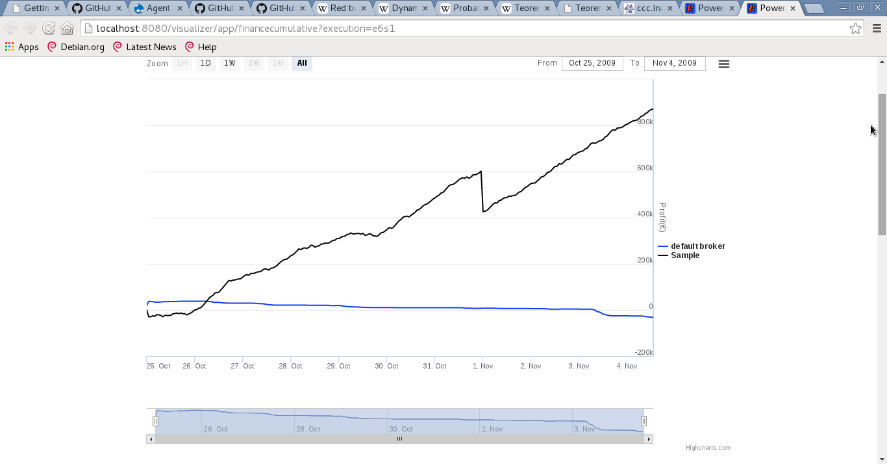
\includegraphics[width=13cm]{img/visualizadorWebResultados.png}
	\caption{Visualizador web de resultados de la simulación.}
	\label{fig:visualizadorWebResultados}
\end{figure}

En la figura \ref{fig:visualizadorWebResultados} el eje $x$ representa el tiempo y el eje $y$ representa la ganancia del broker correspondiente, podemos ver como el Sample broker (el broker que se ejecutó desde NetBeans) inicio con menos ganancias pero conforme
transcurrió el tiempo le gano por mucho al default broker (el broker por defecto que tiene el simulador el cual no ejecuta ninguna estrategia), de igual manera, si hubiera más brokers conectados al servidor estos aparecerían en el gráfico.

Estos resultados de la simulación se guardan además en la carpeta log, que está en la raíz del proyecto, en los archivos \texttt{powertac-sim-0.state} y \texttt{powertac-sim-0.trace}, y cada vez que se corre una simulación el número que en esta primera prueba fue 0, va aumentando.

\section{Estudio de métodos de regresión}
El objetivo es este proyecto es mejorar el broker del INAOE COLDPower, implementando nuevas técnicas que permitan predecir mejor el clima y los patrones de consumo de energía de la población para tomar mejores decisiones y mejorar el rendimiento del broker (aumentar las ganancias en las simulaciones); para llegar a esto fue necesario primero estudiar diversas técnicas de predicción como parte del desarrollo del proyecto, empezando por análisis de regresión. En esta parte del proyecto se llego al siguiente resumen.

Dentro del análisis de regresión hay dos modelos simples por los cuales se
empezó: La regresión lineal y polinomial.

\subsection{Regresión lineal}
El análisis de regresión lineal nos puede ayudar a conocer 3 cosas:

\begin{enumerate}
	\item Si las variables independientes están relacionadas con la variable dependiente, o ayudan a explicar los cambios en la variable dependiente.
	\item Determinar que variables en particular son predictores significativos de la variable dependiente y de qué manera la afectan, la manera en que una variable $x_i$ afecta a la variable dependiente está dada por su coeficiente $\beta_i$ en el modelo generado.
	\item Generar un modelo que muestre como el conjunto de variables predictoras o independientes, pueden ser usadas para predecir valores desconocidos de la variable dependiente y así poder hacer pronósticos. Este modelo naturalmente esta expresado en una ecuación, la cual es una combinación lineal del conjunto de variables independientes.
\end{enumerate}

El estudio de esta técnica fue útil para entender los métodos de regresión en general, ya que es la forma más simple y algunas otras técnicas son parecidas a esta o incluso se basan en ella, como la regresión polinomial, y esta fue el primer tipo de análisis de regresión en estudiarse rigurosamente y en ser usado extensamente en aplicaciones prácticas \cite{XYanLinearRegressionAnalysis}.
Esto es porque los modelos que dependen linealmente de sus variables son más fáciles de ajustar que modelos que son no lineales en cuanto a la relación de sus parámetros y porque las propiedades estadísticas de los estimadores resultantes son más fáciles de determinar.

\subsection{Regresión polinomial}
Como extensión al algoritmo de regresión lineal, se estudió también el análisis de regresión polinomial y su relación con la regresión lineal, que aunque sirve para describir un modelo donde las variables son no lineales (un polinomio), los parámetros a encontrar son lineales.

Por ejemplo, considere una situación en donde una pequeña pelota se lanza al aire y se miden las alturas $h_i$ mientras haciende, durante varios momentos $t_j$. 
Los valores medidos están en la figura \ref{tab:valoresMedidos}. 
El modelo matemático que describe este fenómeno físico nos dice que, ignorando la resistencia del viento, la relación puede ser modelada como:
$$h_i = \beta_1 t_i + \beta_2 t_i^{2} + \varepsilon_i$$
\begin{table}[!h]
	\begin{center}
		\begin{tabular}{|p{2.5cm}|p{2.5cm}|}\hline
			$t_i$ & $h_1$ \\ \hline
				1 & 2 	\\ \hline
				2 & 6	\\\hline
				3 & 12  \\\hline
				4 & 20  \\\hline
				5 & 30  \\\hline
		\end{tabular}			
	\end{center}
	\caption{Valores medidos.}
	\label{tab:valoresMedidos}
\end{table}


Donde $\beta_1$ determina la velocidad inicial de la pelota, $\beta_2$ es proporcional a la constante de gravitación y $\varepsilon_i$ es debido a los errores de medición y/o a la resistencia del viento.
La regresión lineal puede ser usada para estimar los valores de $\beta_1$ y $\beta_2$  a partir de los datos medidos, aunque los datos solo sean dos variables $h_i$ y $t_i$ , solo que en esta tabla de datos de una variable independiente ($t_i$) se extiende a una tabla de datos con dos variables independientes ($t_i$ y $t_i^{2}$), esta transformación de un modelo de $n$ variables independientes a uno con $n*e$ variables independientes, donde $e$ es el grado del polinomio (el exponente más grande). En este caso $n=1$ ya que disponía de solo una variable independiente, y $e=2$ ya que el grado del polinomio que describe el modelo deseado es cuadrático. Este nuevo modelo se representa en la figura \ref{tab:transformacionModelo}.
% si da tiempo cambiar esto por poner las tablas en dos columnas
\begin{table}[!h]  
	\begin{center}
		\begin{tabular}{|p{2.5cm}|p{2.5cm}|p{2.5cm}|}\hline
				$t_i$ & $t_i^{2}$ & $h_1$  \\ \hline
				1 & 1 & 2 	\\ \hline
				2 & 4 & 6	\\\hline
				3 & 9 & 12  \\\hline
				4 & 16& 20  \\\hline
				5 & 25& 30   \\\hline
		\end{tabular}			
	\end{center}
	\caption{ Transformación del modelo de la tabla de la figura \ref{tab:valoresMedidos}}
	\label{tab:transformacionModelo}
\end{table}

Al aplicar regresión lineal a los datos de la tabla de la figura \ref{tab:transformacionModelo} se obtiene una regresión
polinomial de modelo original representado en la tabla de la figura \ref{tab:valoresMedidos}. 
Este método de transformar el modelo para aplicar una regresión polinomial, se usó en la actividad de Implementación de regresión polinomial en la página \pageref{}, a su ves, mas adelante se usa un método parecido a este para hacer análisis de series de tiempo, el cual esta encapsulado en la clase \texttt{WekaForecaster}, parecido en el sentido de que se toma un modelo y se le agregan variables transformándolo en otro modelo que se puede aprender por otro algoritmo de regresión o clasificación cualquiera de la librería weka.

\subsection{Estudio de redes bayesianas}
l estudio de redes bayesianas es necesario ya que se usara este modelo probabilístico como técnica de predicción, más específicamente las redes bayesianas dinámicas, las cuales surgen a partir de las redes bayesianas. Una red bayesiana dinámica o temporal es un modelo estadístico y estocástico que amplía el concepto de red bayesiana.

A diferencia de este último, una red bayesiana dinámica puede representar la evolución de variables aleatorias basándose en una secuencia discreta, por ejemplo, pasos de tiempo. 
El término dinámico caracteriza el sistema modelado, no la red que no cambia.

Un ejemplo de una red bayesiana sería en el diagnóstico médico, para determinar la probabilidad de un paciente que tiene una enfermedad con base en los síntomas. En la figura \ref{fig:redBayesianaDiagnostico} se muestra un ejemplo de una red bayesiana que modela un diagnóstico médico con base de los síntomas.

\begin{figure}[h]
	\centering
	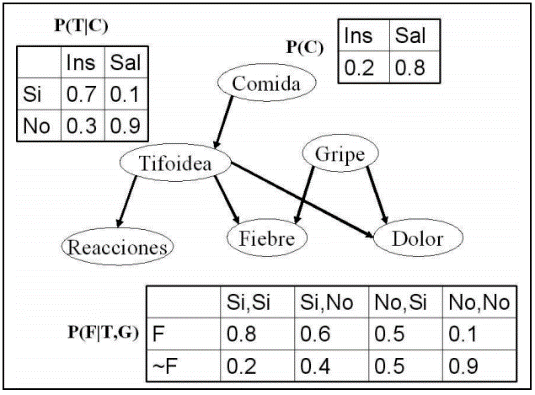
\includegraphics[width=13cm]{img/redBayesianaDiagnostico.png}
	\caption{Red bayesiana que modela un problema de diagnóstico médico.}
	\label{fig:redBayesianaDiagnostico}
\end{figure}

\section{Implementación de métodos de regresión usando la librería weka}

Parte de las actividades futuras es crear un software de pronóstico de producción de energía y pronóstico de consumo de energía que después se adaptara al broker para que este pueda tomar mejores decisiones, para esto se implementaran varios algoritmos de regresión y clasificación que están en la librería weka, por lo que el primer paso hacia llegar al este objetivo es aprender a usar la librería weka.

\subsection{Librería weka}
Weka es una colección de algoritmos del área de machine learning, para tareas de minería de datos. Estos algoritmos pueden ya sea aplicarse directamente a un conjunto de datos, o llamarse desde código java mediante la API de weka.
Weka contiene herramientas para el preprocesado de datos, clasificación, regresión, clusterización, reglas de asociación y visualización. También está bien adaptado para el desarrollo de nuevos esquemas de machine learning. 

El nombre proviene de un ave no voladora de naturaleza inquisitiva que vive solamente en la isla de Nueva Zelanda.

Weka es un software de código abierto, bajo la licencia GNU General Public License.

En este periodo se hicieron varias pruebas con la librería weka, empezando por pruebas desde consola, como la de la figura \ref{}, con los datos de ejemplo que trae la librería weka, y después se desarrolló un proyecto en java que hace uso de la API de esta librería.




